\chapter{About}
\graphicspath{{Appendix4/}}
\section*{About Me}
\textbf{Tsinghua University}\\
Undergraduate | August, 2014 - \\
\textbf{University of Tokyo}\\
Visiting student researcher|June,2017 - August, 2017\\
\begin{figure}[htbp!] 
\centering    
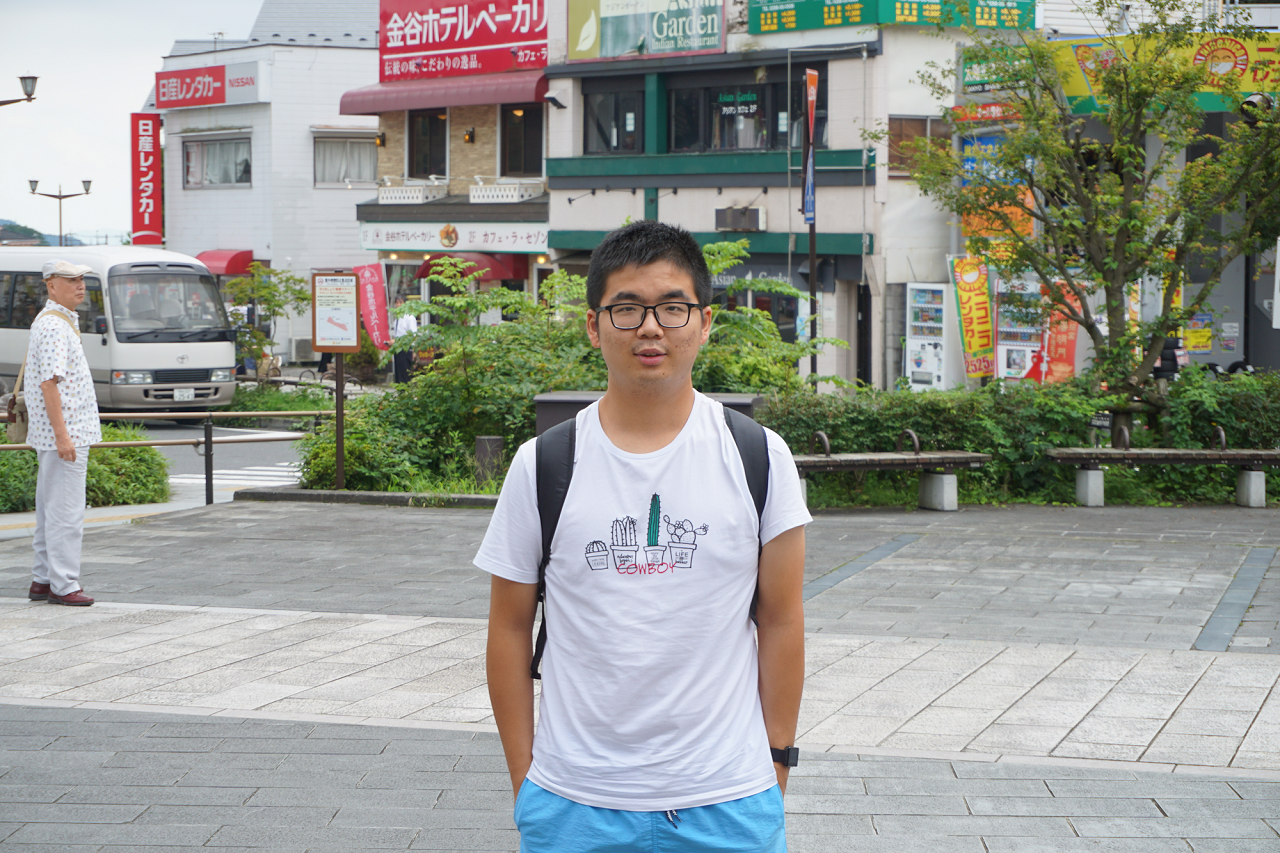
\includegraphics[width=0.8\textwidth]{xiao.png}
\caption[Xiao Feiyu]{Xiao Feiyu}
%\label{fig:cell}
\end{figure}
I show a great interest and passion in Quantum and Statistical Mechanics and have oriented my research focus on them, especially in nano materials. I've selected several related courses about it, such as Statistical Mechanics and Quantum Mechanics. During the recent months, I am doing some projects about phonon transport in nanofilms, especially their properties in interfaces. \\
\textbf{My Research}\\
I conduct my ORIC study under Prof. Bingyang Cao's guidance to learn the MC method to simulate the nano-film heat condution and do the optimization.This summer from June to Angust, I worked at Prof.Junichiro Shiomi 's Lab in Mechanical Engineering of University of Tokyo. My research topic was phonon properties at the interface using atomistic green function approach. And we also study the design and optimization of nanostructures via Bayesain optimization.\\
Tel: +86-17888830399\\
Email: xiao-14@mails.tsinghua.edu.cn\\


\section*{Supervisor: Prof. Bingyang Cao}
\begin{figure}[htbp!] 
\centering    
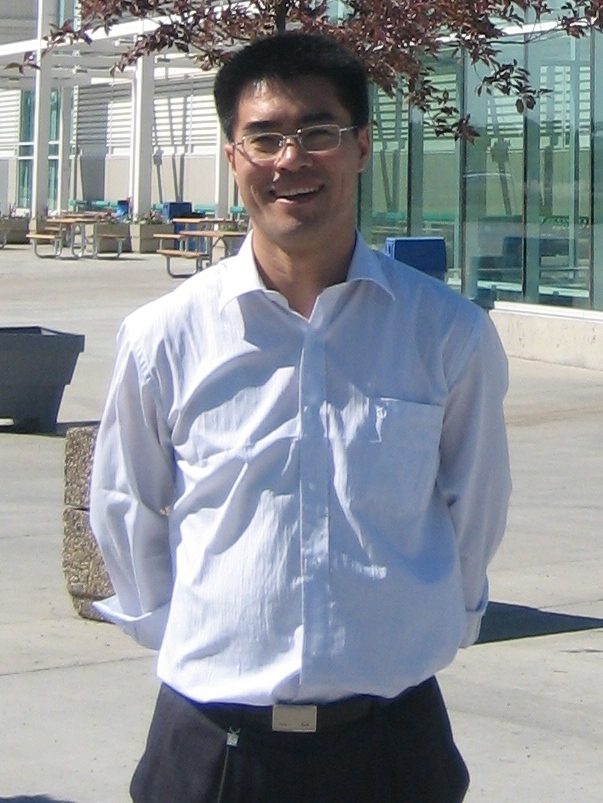
\includegraphics[width=0.3\textwidth]{Cao.png}
\caption[Prof. Bingyang Cao]{Prof. Bingyang Cao}
%\label{fig:cell}
\end{figure}
Prof. Bingyang Cao, leader of the Heatenergists Group (HEG), is also vice dean in School of Aerospace Engineering, Tsinghua University, China. His research areas are mainly focused on: (1) Non-Fourier heat transport and thermophysical properties of micro/nano-structures, including nanofilms, nanowires, nanotubes, graphene, polymer chains etc; (2) Thermal smart materials and nanocomposites with tunable or high thermal conductivity, and their applications in energy or micro/nano-electrics cooling areas; (3) Thermal management technology and theory in advanced technologies, such as nanoenergy, integrated circuits, MEMS/NEMS, laser, spacecrafts. Our work is interdisciplinary and involved in energy, aerospace, thermophysics, micro/nanofluidics and material sciences. HEG has established, as well as is seeking, extensive collaborations in research and development with universities, institutes and industries.\\
Bingyang Cao received his B.S. (1998) and M.S. (2001) from Shandong University, and Ph.D. (2005) in engineering thermophysics from Tsinghua University. He then joined Tsinghua University in 2005, and is currently a full professor and vice dean at the School of Aerospace Engineering, Tsinghua University. He also worked in Kyushu University (2005), The Hong Kong Polytechnic University (2006) and The University of Brighton (2007,2010) as a visiting professor. He has published over 100 SCI-indexed journal papers and serves as editorial board member of Scientific Reports, PLOS One, Advances in Materials Research etc. He won the New Century Excellent Talents of MOE (2011), Excellent Young Scientist Award of NSFC (2013), Zhonghua-Wu Outstanding Young Scholar Award of ETPC (2014), APL Top Reviewer Award (2017). His current research interests include non-Fourier heat conduction and thermophysical properties of nanostructures, thermal smart materials and nanocomposites, advanced thermal management technologies etc.\\
Office: Room N807, Meng Minwei S/T Building\\
Tel: +86-10-6279-4531\\
Email: caoby@tsinghua.edu.cn\\
\section*{Prof. Junichiro Shiomi}
\begin{figure}[htbp!] 
\centering    
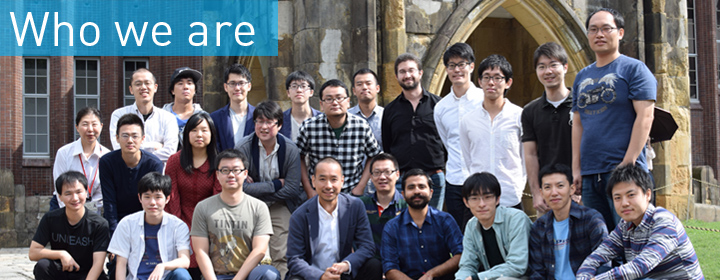
\includegraphics[width=0.8\textwidth]{shiomi.png}
\caption[Prof. Junichiro Shiomi]{Prof. Junichiro Shiomi's lab}
%\label{fig:cell}
\end{figure}
 Prof. Junichiro Shiomi received the B.E. (1999) from Tohoku University, and Ph. D. (2004) from Royal Institute of Technology (KTH), Sweden. He is currently a Professor in Department of Mechanical Engineering, The University of Tokyo. His research interests include heat conduction of nanomaterials, polymer composites, and thermoelectrics, phase change and fluidics in nanoscale, interfacial thermofluid dynamics, thermal convections, and materials informatics. He is a recipient of the Zeldovich Medal from the Committee on Space Research, Young Scientists' Prize, the Commendation for Science and Technology by the Minister of Educational, Culture, Sports, Science and Technology, and the Academic award of Heat Transfer Society of Japan. \\ 
Email: shiomi@photon.t.u-tokyo.ac.jp

